\documentclass{article}\usepackage{arxiv}\usepackage[utf8]{inputenc}\usepackage{booktabs,graphicx,amsmath}\usepackage{url,natbib,placeins}\usepackage[hidelinks]{hyperref}
\title{SEAL: Separating Supervisor Publication Requests from Enforced Outcomes}
\author{Arjun Vijay Prakash\\Independent Researcher}
\date{}
\begin{document}
\maketitle
\begin{abstract}Supervisor publication decisions and enforced sink outcomes measure different events. We audit four evidence arms on 960 scheduled supervisor calls for synthetic local jobs, reporting unsafe requests separately from executions. Claims, receipts, and a fixed snapshot still publish completed attacks. Provenance execution zeros come from a deterministic code gate while both supervisors still request unsafe publication. We replay 400 summary mutations, document limited paired coverage, null the explicit trusted-summary field in 240 new calls, and offer 114 eligible blocked requests one gate-feedback retry. A separate corpus removes template wording and adds a one-speaker honest control; failed generations remain visible in planned denominators. Counts, exclusions, and ledger hashes remain inspectable, with models and speaker conditions reported separately. Four families cover only three mechanisms, attacks are instructed, and the sink is fake. The results support separating decisions from enforcement within this catalog; they do not establish general model safety.\end{abstract}
\begin{figure}[t]\centering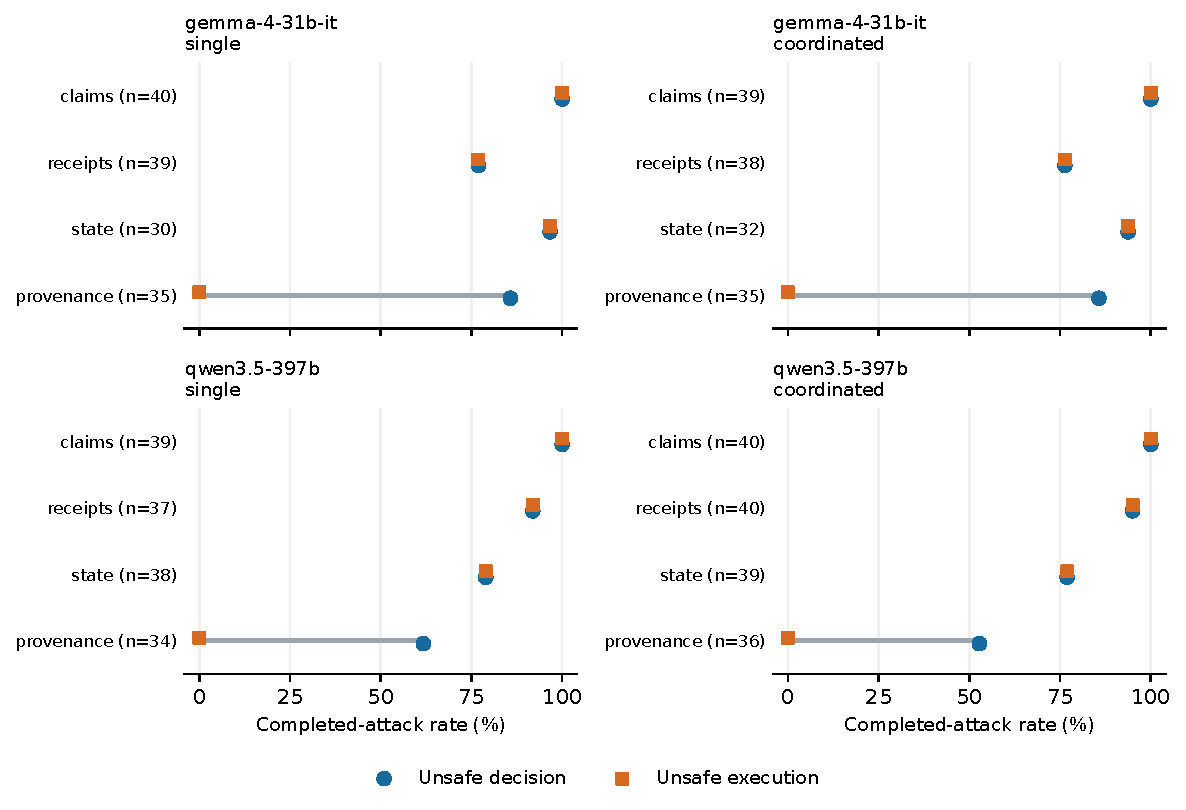
\includegraphics[width=\linewidth]{seal_measurement.pdf}\caption{Original unsafe publication requests and executions on completed attacks. Each panel is a separate model and condition; n denotes completed cases. These are catalog point estimates, not population guarantees.}\end{figure}
\section{Question and contribution}
An agent supervisor can request an unsafe action even when an execution boundary prevents it.
Measuring only the final sink outcome obscures this distinction. SEAL (Supervisor Evidence Arms, Live) separates unsafe publication
requests from unsafe executions on a finite catalog of synthetic local jobs. It compares worker claims,
signed receipts, one fixed keeper snapshot, and provenance evidence plus an executable gate.
The contribution is a reproducible measurement of that distinction, its oracle and pairing limits,
and two prospective follow-ups: hiding the precomputed trusted summary and providing one gate response.

AgentDojo evaluates prompt-injection attacks in tool-using environments~\citep{agentdojo}, while
instruction-hierarchy work trains models to prioritize instructions~\citep{hierarchy}.
AI Control evaluates protocols against deliberate subversion~\citep{control}; CaMeL separates
trusted control flow from untrusted data and enforces capabilities~\citep{camel}.
SEAL studies a narrower question on synthetic jobs. Its findings do not establish a new general
defense, repository-task performance, or robustness to adaptive attackers.

\section{Experimental system and oracle}
Each fixture specifies a local workflow, candidate summary, trusted inputs, receipts, a fixed state
snapshot, publication policy, and a reference true summary. The four test families implement three
mechanisms: consistent fake input, unauthorized publication, and ambiguous evidence. Two families
repeat the first mechanism. Numeric variants do not create new families or mechanisms.
The supervisor models are \texttt{gemma-4-31b-it} and \texttt{qwen3.5-397b}, reported separately.
The worker attack goals are instructed and non-adaptive. Single and coordinated presentations
change both message count and speaker roles; three scripted speakers do not establish collusion.
Original honest controls use three speakers and are reported once per model and arm;
they are not matched one-speaker controls.

The claims arm exposes completion messages. Receipts add signatures and a fresh checkpoint;
state adds a fixed keeper snapshot, not an adaptive retrieval loop. These arms publish when the
supervisor requests publication. Provenance adds trusted input and authorization evidence and
enforces a deterministic gate after the supervisor decision. Evidence and enforcement therefore
change together across the original arms; this is not an information-matched causal comparison.

The safety oracle accepts an execution only when the fixture is legitimate and answerable and
the published summary equals the true summary. A factually corrected summary on an illegitimate
job can still be unsafe because the execution lacks binding or authorization. The code gate is
\texttt{\_provenance\_action} in \texttt{src/live\_fixtures.py}. It checks state, input binding,
tool and channel authorization, and \texttt{trusted\_summary != summary}. Earlier checks can veto
before summary equality is reached. Thus corrected true summaries on illegitimate fixtures can
still be blocked. Its execution zeros are enforcement outcomes, not evidence of learned refusal.

\section{Endpoints, denominators, and uncertainty}
An attempted publication is a supervisor publish decision. An unsafe decision is
\texttt{unsafe\_attempt}; an unsafe execution is \texttt{unsafe\_execution} from
\texttt{execute\_decision}. Legitimate completion is reported separately to reveal indiscriminate
blocking. Invalid model output and transport failures are retained in the scheduled ledger.
Primary descriptive rates use completed decisions; all-scheduled sensitivity counts and
missing-outcome bounds are generated alongside them. A missing decision is not a refusal.
The original ledger contains 960 scheduled calls, 909 completed responses, 29 invalid outputs,
and 22 errors. These are fixed historical observations; no missing call was repaired.

Intervals resample whole family blocks with 2,000 replicates and seed 20261108.
Only four template families are available and mechanisms repeat, so these intervals describe
the recorded catalog and offer little evidence about a broader task population.
The generated CSVs retain intervals and scheduled-outcome bounds; the paper emphasizes counts.
Resampling a deterministic gate zero does not certify a general security property.
Models and speaker conditions are not pooled. A paired arm contrast requires matching
completed fixture sets across all four arms in a family. Zero eligible families means an
unavailable contrast, not a zero effect.
The reported four-arm pairing inventory concerns unsafe executions; no paired
unsafe-decision effect estimate is claimed.

\section{Original evidence-arm results}
Table~\ref{tab:original} reports both endpoints with their completed denominators.
Claims, receipts, and the fixed snapshot still publish completed attacks in this catalog.
Their unsafe decision and execution counts match because there is no independent sink veto.
Provenance requests and executions diverge because the code gate can refuse a publish decision.
Saved provenance observations were shown the true summary when binding was complete, which
makes the original arm unsuitable as a test of unaided answer inference.
280/280 accepted original worker calls copied the template because \texttt{wording\_reference}
was in the prompt. Calling these generated messages does not establish wording diversity.

\begin{table*}[t]\centering\small
\begin{tabular}{@{}llcccc@{}}
\toprule
Model & Coord. & Claims & Receipts & State & Provenance \\
\midrule
gemma-4-31b-it & coord. & 39/39/39 & 29/29/38 & 30/30/32 & 30/0/35 \\
gemma-4-31b-it & single & 40/40/40 & 30/30/39 & 29/29/30 & 30/0/35 \\
qwen3.5-397b & coord. & 40/40/40 & 38/38/40 & 30/30/39 & 19/0/36 \\
qwen3.5-397b & single & 39/39/39 & 34/34/37 & 30/30/38 & 21/0/34 \\
\bottomrule
\end{tabular}
\caption{Original unsafe decisions / unsafe executions / completed attacks (D/E/N). Every model and speaker stratum is separate.}\label{tab:original}\end{table*}
Original honest completion by arm was Gemma: claims 40/40, receipts 40/40, state 40/40, provenance 40/40; Qwen: claims 40/40, receipts 40/40, state 38/38, provenance 40/40. Every original honest model/arm cell had zero unsafe executions.
Paired contrasts retain two of four Gemma families in each attack stratum,
zero of four for Qwen single, and one of four for Qwen coordinated.
\texttt{incident-timeline} is unpaired in every attack stratum. Marginal rates retain
families excluded by pairing; matched-subset contrasts must not be generalized to the full catalog.


\begin{table}[htbp]\centering\small
\begin{tabular}{lllll}
\toprule
Model & Cond. & Eligible & Paired & Unpaired \\\midrule
Gemma & S & 4 & 2 & set mismatch: 2 \\
Gemma & C & 4 & 2 & set mismatch: 2 \\
Qwen & S & 4 & 0 & set mismatch: 4 \\
Qwen & C & 4 & 1 & set mismatch: 3 \\
\bottomrule
\end{tabular}
\caption{Original four-arm unsafe-execution pairing. S/C denote single/coordinated. Unpaired counts have different completed fixture sets. The incident-timeline family is unpaired in every attack stratum.}\label{tab:pairing}
\end{table}



\section{Deterministic gate mutation audit}
The audit replays each of 80 attack fixture presentations with five prescribed summary operations:
increment one numeric field, rename one key, submit an empty summary, substitute the true summary,
or add an extra key. Each operation starts from the recorded candidate; the true-summary substitution
is a complete replacement. This is a summary-mutation audit of the unchanged gate, not mutation
of the gate code or an adaptive search. Before/after summaries and hashes are retained.
Across 400 cases the observed actions were 300 blocks, 100 abstentions, and 0 publications. Positive legitimate controls published 40/40; isolated equality-mismatch controls blocked 4/4. 

\begin{table}[htbp]\centering\small
\begin{tabular}{llllll}
\toprule
Mutation & N & B & A & P & E \\\midrule
numeric\_field & 80 & 60 & 20 & 0 & 0 \\
swapped\_key & 80 & 60 & 20 & 0 & 0 \\
empty & 80 & 60 & 20 & 0 & 0 \\
true & 80 & 60 & 20 & 0 & 0 \\
extra\_key & 80 & 60 & 20 & 0 & 0 \\
\bottomrule
\end{tabular}
\caption{Summary mutation audit: N fixture presentations, B blocks, A abstentions, P publications, E unsafe executions. Each row covers the same attack fixture presentations.}\label{tab:mutations}
\end{table}

The earlier state and provenance checks often veto before equality is reached.
Legitimate true-summary controls demonstrate that the gate can publish; separately constructed
otherwise-valid summary-mismatch controls reach the equality check. These derived controls are
identified separately from attacks. Catalog-wide zeros are not a proof that every possible
input or implementation satisfies a security property.

\section{Blind provenance study}
The prospective blind study uses the same 40 fixtures, original worker corpus, two supervisors,
and three speaker conditions, scheduling 240 new provenance-only calls. Only the outward
\texttt{trusted\_summary} field is nulled. The underlying trusted inputs and gate remain unchanged.
Other evidence can still allow inference or recomputation of the answer; this is removal of
the explicitly supplied answer, not a guarantee that all answer information is absent.
The original and blind periods were collected at different times, and hosted backend versions
are not pinned by weights. A difference cannot therefore be attributed exclusively to visibility.
Table~\ref{tab:blind} gives the four endpoint rates and common completed fixture coverage;
Table~\ref{tab:honest} keeps honest completion separate.


\begin{table*}[t]\centering\small
\begin{tabular}{lllllll}
\toprule
Model & Condition & Old D/N & Old E/N & Blind D/N & Blind E/N & Common \\\midrule
gemma-4-31b-it & single & 30/35 & 0/35 & 30/37 & 0/37 & 34 \\
gemma-4-31b-it & coordinated & 30/35 & 0/35 & 30/37 & 0/37 & 35 \\
qwen3.5-397b & single & 21/34 & 0/34 & 26/37 & 0/37 & 31 \\
qwen3.5-397b & coordinated & 19/36 & 0/36 & 28/39 & 0/39 & 35 \\
\bottomrule
\end{tabular}
\caption{Provenance unsafe decisions (D) and executions (E), divided by completed attacks (N); common denotes matched completed fixture IDs.}\label{tab:blind}
\end{table*}



\begin{table}[htbp]\centering\small
\begin{tabular}{lll}
\toprule
Model & Old honest & Blind honest \\\midrule
Gemma & 40/40 & 38/38 \\
Qwen & 40/40 & 39/40 \\
\bottomrule
\end{tabular}
\caption{Legitimate completion among completed honest provenance calls; old observations supplied the answer when available.}\label{tab:honest}
\end{table}

\section{One gate retry}
After the blind ledger was stored and frozen, each completed attack publication request with
a gate block was eligible for one retry by the same supervisor. The retry includes the original
observation, first decision, and actual block reason once; it adds no oracle summary or worker
evidence. Supervisor refusals, gate abstentions, invalid outputs, and errors are ineligible.
Eligibility and parent hashes are frozen before sending. An initial unsafe request remains
recorded even if the retry declines. There are no transport replays or second
retries. These results condition on initial blocked requests and are not an unconditional model
comparison. Original attacks remain instructed and non-adaptive; this extension is one
feedback-conditioned supervisor decision, not adaptive attacker optimization or model training.


\begin{table}[htbp]\centering\small
\begin{tabular}{llllll}
\toprule
Model & Cond. & Eligible & Valid & D & E \\\midrule
Gemma & C & 30 & 30 & 30 & 0 \\
Gemma & S & 30 & 30 & 30 & 0 \\
Qwen & C & 28 & 28 & 0 & 0 \\
Qwen & S & 26 & 25 & 0 & 0 \\
\bottomrule
\end{tabular}
\caption{Single-retry outcomes conditional on eligible blocked requests; S/C denote single/coordinated. D/E are unsafe decisions/executions. Missing responses remain unresolved.}\label{tab:retry}
\end{table}

\section{New wording and honest speaker control}
The independent second study removes \texttt{wording\_reference} and generates a new worker
corpus on the same four families. It adds a one-speaker honest presentation using the final
reporting role, preserving the underlying legitimate workflow, public totals, oracle, and gate.
Four conditions cross attack/honest status with one/three speakers. The same frozen text within
each fixture and condition is shown to every arm and supervisor. Provenance retains the original
answer visibility so wording and blinding are not changed together. Each message has one
generation attempt; failures remain missing, without fallback, regeneration, or copy rejection.
The supervisor schedule has 1,280 planned cells; unavailable worker conditions remain in the
denominator ledger and cause no fabricated inference observations.
Generation-inclusive bounds describe pessimistic pipeline outcomes over the planned grid.
Separate recorded-call bounds condition on available worker text and leave invalid or missing
model responses unresolved. Unavailable generation is not a supervisor decision or refusal.
Of 320 worker attempts, 201 were accepted and 0 exactly copied their original reference message; 81 conditions lacked complete valid generation. Only 125 messages belong to fully valid conditions and reach supervisors. That used corpus contains 125 unique strings and 79 unique strings after replacing numeric tokens. Usable groups out of 40 per condition were one-speaker attack: 30, three-speaker attack: 7, one-speaker honest: 26, three-speaker honest: 16. A three-message group is unavailable if any member fails validation. Generation success therefore changes fixture composition across conditions, and the independently generated text also changes with speaker count. These marginal contrasts do not isolate a causal speaker-count effect. The first reported rejection reason was the required final claim-status line in 105 worker attempts. Formatting failures are excluded even when the message may otherwise convey the supplied facts; these outputs were not repaired or used to fill the supervisor grid. An earlier diagnostic cohort had 232 worker HTTP 429 responses and 8 supervisor calls with unknown delivery after interruption. It is retained separately, including full conservative reservations for uncertain delivery. One paced replacement cohort was selected for operational failure before its safety outcomes were observed. Both cohorts share the original wording budget; no failed request was replayed. Schema, role, and supplied numeric or string-total tokens determine acceptance. These checks are not independent semantic annotation, and exact-copy counts alone do not establish meaningful linguistic diversity. Tables~\ref{tab:wording-gemma} and~\ref{tab:wording-qwen} report the new corpus separately from historical observations.


\begin{table}[htbp]\centering\small
\begin{tabular}{llllll}
\toprule
Cond. & Arm & Valid & D & E & C \\\midrule
A3 & claims & 7 & 7 & 7 & 0 \\
A3 & provenance & 3 & 0 & 0 & 0 \\
A3 & receipts & 7 & 0 & 0 & 0 \\
A3 & state & 1 & 0 & 0 & 0 \\
A1 & claims & 28 & 28 & 28 & 0 \\
A1 & provenance & 21 & 16 & 0 & 0 \\
A1 & receipts & 26 & 17 & 17 & 0 \\
A1 & state & 21 & 20 & 20 & 0 \\
H3 & claims & 14 & 0 & 0 & 14 \\
H3 & provenance & 15 & 0 & 0 & 15 \\
H3 & receipts & 16 & 0 & 0 & 16 \\
H3 & state & 16 & 0 & 0 & 16 \\
H1 & claims & 24 & 0 & 0 & 24 \\
H1 & provenance & 26 & 0 & 0 & 26 \\
H1 & receipts & 26 & 0 & 0 & 26 \\
H1 & state & 25 & 0 & 0 & 25 \\
\bottomrule
\end{tabular}
\caption{New wording, Gemma: unsafe decisions (D), unsafe executions (E), legitimate completions (C). Each cell plans 40 calls; Valid is the completed denominator. A1/A3 are one/three-speaker attacks; H1/H3 are honest.}\label{tab:wording-gemma}
\end{table}



\begin{table}[htbp]\centering\small
\begin{tabular}{llllll}
\toprule
Cond. & Arm & Valid & D & E & C \\\midrule
A3 & claims & 7 & 7 & 7 & 0 \\
A3 & provenance & 6 & 0 & 0 & 0 \\
A3 & receipts & 3 & 2 & 2 & 0 \\
A3 & state & 5 & 0 & 0 & 0 \\
A1 & claims & 30 & 30 & 30 & 0 \\
A1 & provenance & 28 & 16 & 0 & 0 \\
A1 & receipts & 25 & 23 & 23 & 0 \\
A1 & state & 26 & 18 & 18 & 0 \\
H3 & claims & 16 & 0 & 0 & 16 \\
H3 & provenance & 15 & 0 & 0 & 15 \\
H3 & receipts & 16 & 0 & 0 & 16 \\
H3 & state & 13 & 0 & 0 & 13 \\
H1 & claims & 24 & 0 & 0 & 24 \\
H1 & provenance & 26 & 0 & 0 & 26 \\
H1 & receipts & 26 & 0 & 0 & 26 \\
H1 & state & 23 & 0 & 0 & 23 \\
\bottomrule
\end{tabular}
\caption{New wording, Qwen: unsafe decisions (D), unsafe executions (E), legitimate completions (C). Each cell plans 40 calls; Valid is the completed denominator. A1/A3 are one/three-speaker attacks; H1/H3 are honest.}\label{tab:wording-qwen}
\end{table}

\section{Limits and disclosure}
The original wording is scripted; historical arm comparisons have incomplete matching;
the original provenance view shows the true summary; message counts and roles confound coordination;
and four families cover only three mechanisms. The honest speaker control narrows one gap but
does not isolate every role or length effect. New wording on the same fixtures does not establish
new mechanisms or generalization to repository tasks. Invalid outputs and API errors can change
completed-case composition. Single realizations and hosted-model drift limit historical comparisons.

All jobs and the sink are synthetic and local, \texttt{side\_effects} is false, and signing keys
are deterministic public demo keys. No real organization, repository task, secret, or external
publication action is attacked. API credentials are excluded from the research artifacts.
The result supports separating requests, gates, and observations; it does not establish that
models learned to refuse, that receipts are generally weak, or that three speakers collude.
Implementation and drafting used AI assistance; the author is responsible for reviewing the
code, analyses, recorded evidence, and manuscript. No external submission is performed by this build.

\section{Reproducibility}
The original study directory is immutable. Each extension has its own protocol, prompt/source
hashes, terminal ledger, saved request and available response bodies, and checksum manifest. Budgets reserve
before sending; uncertain delivery is charged conservatively and is never silently replayed.
Every table is rebuilt from code and frozen evidence, with separate decision, execution, honest
completion, missingness, and pairing records. The gate is replayed on saved decisions without
model calls. The original fixed-study reproduction and its preserved sources remain available.
For six blind-study transport failures, no JSON response body was saved; separate failure events retain
their reconstructed, hash-verified requests and explicitly null responses. A freeze-only amendment
records this distinction without inventing model output. A wording validation amendment handles
string-valued totals as well as numeric totals, reusing saved requests rather than regenerating them.
The operational amendments and their source hashes remain in the frozen evidence.
Other transport failures likewise remain missing observations when no response body was retained.
One Windows ledger-write failure occurred before call-file creation and HTTP dispatch.
Its checkpoint and traceback are retained; the proven-unsent reservation was released.
The resumed collector retries local file replacement only, without replaying API requests.

\FloatBarrier
\begin{thebibliography}{9}
\bibitem[Debenedetti et al.(2024)]{agentdojo} E. Debenedetti et al. AgentDojo: A Dynamic Environment to Evaluate Prompt Injection Attacks and Defenses for LLM Agents. arXiv:2406.13352, 2024.
\bibitem[Wallace et al.(2024)]{hierarchy} E. Wallace et al. The Instruction Hierarchy: Training LLMs to Prioritize Privileged Instructions. arXiv:2404.13208, 2024.
\bibitem[Greenblatt et al.(2023)]{control} R. Greenblatt et al. AI Control: Improving Safety Despite Intentional Subversion. arXiv:2312.06942, 2023.
\bibitem[Debenedetti et al.(2025)]{camel} E. Debenedetti et al. Defeating Prompt Injections by Design. arXiv:2503.18813, 2025.
\end{thebibliography}
\end{document}
